\documentclass[../review_2.tex]{subfiles}
\graphicspath{{\subfix{../img/}}}
\begin{document}

\chapter{Feinentwurf}\thispagestyle{fancy}

\begin{itemize}
\item falls wir es nicht in ein extra Paket packen, wird hier alles erklärt, was im Root-Ordner liegt. Also Thread (WorkerThread) und das was in main.cpp passiert. Also der Initialisierungskram
\item Außerdem: Klassendiagramm der ganzen Software, ohne Methoden, Attribute, nur die Namen der Klassen und die Beziehungen zwischen den Klassen, vielleicht visuell angeordnet nach Paketen (hübsch mit gestrichelten Linien wenn möglich)\\

\item Initialisierung:
    \begin{itemize}
    \item init\_dpdk (wird im Allgemeinen nicht genauer erklärt)
    \item symmetric rss
    \item Starten von Threads
    \end{itemize}

\end{itemize}

\section{NicManagement}
- Klassendiaramm, doxygen

\section{ConfigurationManagement}
\subsection{Configurator}
Für die Software gibt es eine Konfigurationsdatei, ,,config.json'', welche innerhalb dieser Klasse eingelesen wird und diese Informationen global zur Verfügung stellt. Von der Klasse soll es im ganzen Programmablauf nur ein Objekt geben, damit keine Inkonsistenzen entstehen können. 
\begin{figure}[h]
    \centering
    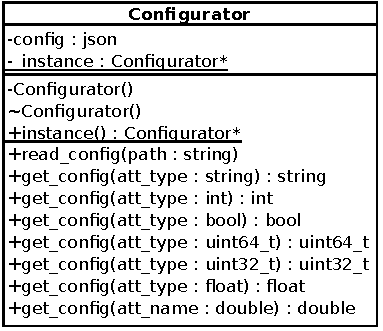
\includegraphics[width=0.98\linewidth]{img/configurator.pdf}
    \caption{Klassendiagramm Configurator}
    \label{Class_Configurator}
\end{figure}
Aufgrund dieser Anforderungen kann ein spezielles Entwurfsmuster verwendet werden, der Singleton. Der Singleton ist ein Erzeugungsmuster, welches automatisch dafür sorgt, dass nur eine Instanz des Configurator existieren kann, und stellt ähnlich globalen Variablen Informationen global dar. Der Vorteil des Singleton diesen gegenüber besteht darin, dass der Singleton nur dann verwendet wird, wenn er wirklich benötigt wird. Die Klasse des Configurator hat nur einen privaten Konstruktor, welcher in der zum Singleton gehörigen Methode der Instanziesierung, verwendet wird. In der ersten Verwendung des Configurators wird die Methode, ,,read\_config()'', zur Einlesung der Daten ausgeführt.Falls die Configurationsdatei nicht findbar ist, so wird eine Exception geworfen, da die Software ohne diese nicht ablaufen kann. Die ausgelesenen Daten werden dann in einem privaten json-Objekt hinterlegt. Hierzu wichtig zu erwähnen ist, dass nlohmann::json verwendet wird. Die Informationen der json-Datei werden über eine Schnittstelle ,,get\_config(Datentyp)'' anderen Klassen zur Verfügung gestellt, wobei es unterschiedliche Methode je nach Datentyp gibt. Der explizite Aufruf des Auslesens erfolgt über die Methode ,,instance()'', mithilfe jener ein Zeiger auf das Configurator-Objekt zurückgegeben wird.


\subsection{Initializer}
Die Klasse Initializer dient dazu, dass grundlegende Initialisierungen für ,,DPDK'' vorgenommen werden, hierzu gibt es die Methode ,,init\_dpdk(int argc, char** argv)''.

\subsection{Thread}
Diese Klasse dient dazu, dass parallele Threads erzeugt werden können, welche dann die gesamte Paketbehandlung des Systems durchlaufen. Hierzu werden jedem Thread zwei PacketContainer übergeben. Ein PacketContainer dient zum annehmen von Paketen welche von außerhalb des Netzwerkes in das Netzwerk kommen und der andere analog dazu mit Paketen, welche von innerhalb des Netzwerkes nach außen sollen. Die run-Methode der Thread-klasse besteht daraus, dass eine bestimmte Anzahl an Paketen gepollt wird mittels der Methode ,,poll\_packets(int number)''. Dies gilt für beide PacketContainer. Nachdem die Pakete behandelt wurden, was innerhalb dieses Pollings passiert, werden die restlichen Pakete nun in jeweilige Richtung weitergeschickt mittels ,,send\_packets()''.

\subsection{Initializer}
Die Klasse Initializer dient dazu, dass grundlegende Initialisierungen für ,,DPDK'' vorgenommen werden, hierzu gibt es die Methode ,,init\_dpdk(int argc, char** argv)''.
\section{PacketDissection}
Die Aufgabe der PacketDissection ist es, Informationen über die zu untersuchenden Pakete bereitzustellen. Zusätzlich wird auch die Kommunikation mit dem NicManagement über die PacketDissection geleitet.

Im Diagramm \ref{Sequenzdiagramm_PacketDissection} wird das Polling von Paketen unter Benutzung des PacketContainers dargestellt. Der PacketContainer fungiert hierbei als zentrales Element, dass den Ablauf steuert.

\begin{figure}
	\centering
	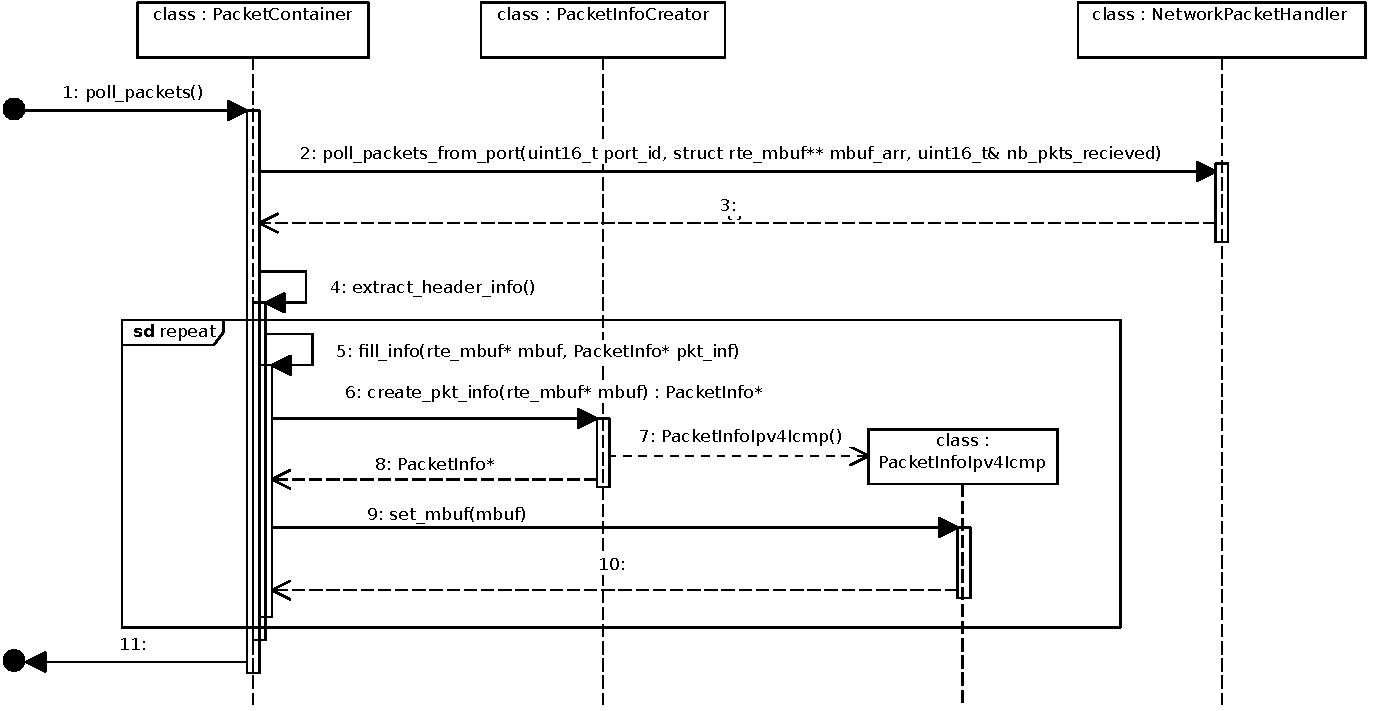
\includegraphics[width=\linewidth]{img/SequenceDiagramPacketDissection2.pdf}
	\caption{Sequenzdiagramm zum polling von Paketen über den PacketContainer}
	\label{Sequenzdiagramm_PacketDissection}
\end{figure}

\subsection{Thread}
Diese Klasse dient dazu, dass parallele Threads erzeugt werden können, welche dann die gesamte Paketbehandlung des Systems durchlaufen. Hierzu werden jedem Thread zwei PacketContainer übergeben. Ein PacketContainer dient zum annehmen von Paketen welche von außerhalb des Netzwerkes in das Netzwerk kommen und der andere analog dazu mit Paketen, welche von innerhalb des Netzwerkes nach außen sollen. Die run-Methode der Thread-klasse besteht daraus, dass eine bestimmte Anzahl an Paketen gepollt wird mittels der Methode ,,poll\_packets(int number)''. Dies gilt für beide PacketContainer. Nachdem die Pakete behandelt wurden, was innerhalb dieses Pollings passiert, werden die restlichen Pakete nun in jeweilige Richtung weitergeschickt mittels ,,send\_packets()''.

\section{PacketDissection}
\subsection{PacketContainer}
DPDK liefert beim Pollen von Paketen ein Array von Pointern auf sogenannte \texttt{mbuf}-Strukturen. Auch beim Senden muss dem Framework ein solches Array übergeben werden, denn die \texttt{mbuf}-Strukturen repräsentieren Pakete innerhalb von DPDK. Um nur die PacketInfo-Objekte durch das Programm reichen zu müssen, wäre das Array von \texttt{mbuf}-Strukturen zu durchlaufen und die Pointer jeweils in die PacketInfo-Objekte zu schreiben. Ein \texttt{mbuf} (Paket) gehört dabei genau einer PacketInfo. Wenn dann am Ende der Pipeline Pakete gesendet werden, müssten die Pointer der \texttt{mbuf}-Strukturen den PacketInfo-Objekten wieder entnommen und in ein Array geschrieben werden. Dies ist überflüssiger Aufwand, da es möglich ist, das empfangene \texttt{mbuf}-Array beizubehalten. Dies setzt der PacketContainer um.

\begin{figure}
	\centering
	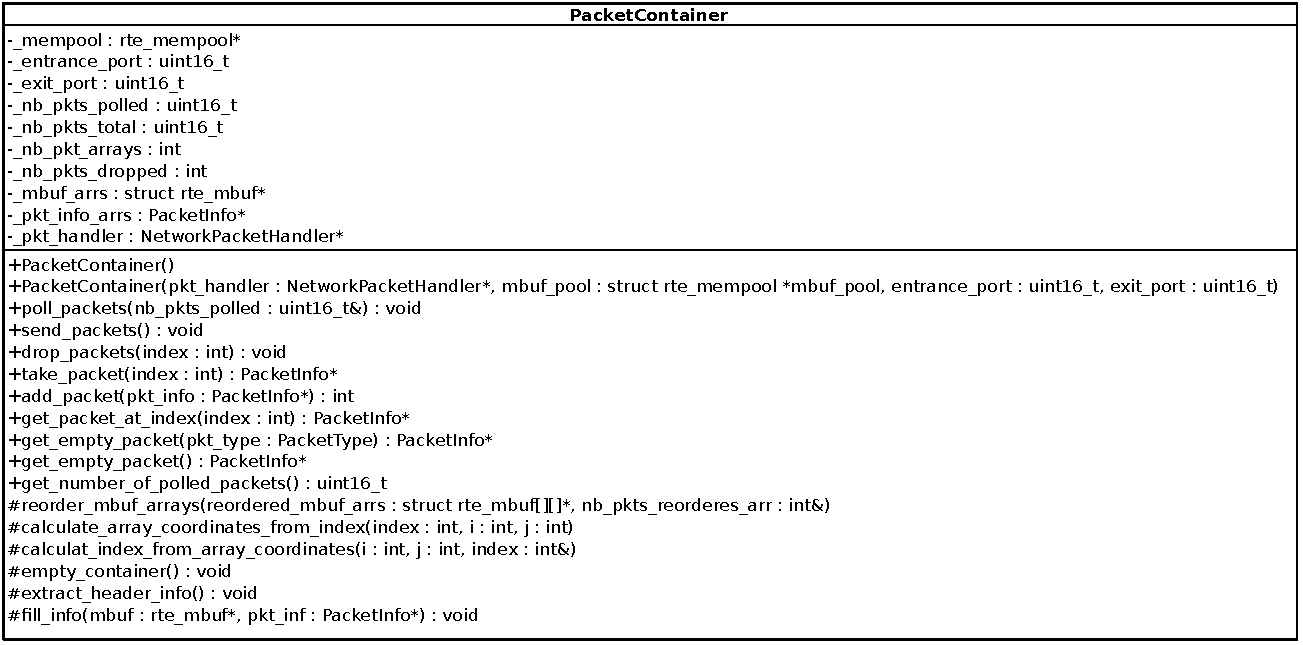
\includegraphics[width=\linewidth]{img/PacketContainerClass.pdf}
	\caption{Klassendiagramm PacketContainer}
	\label{Klassendiagramm_PacketContainer}
\end{figure}

Der PacketContainer ist keine aktive Klasse und wird aufgerufen um spezielle, in Dagramm \ref{Klassendiagramm_Packet} angegebene Aufgaben umzusetzen. Eine dieser Aufgaben ist das polling von Paketen, der Ablauf wird im Sequenzdiagramm \ref{Sequenzdiagramm_PacketDissection} dargestellt. Eine weitere Aufgabe ist das verwerfen von Paketen, welches durch \textit{drop\_packet(int index)} umgesetzt wird. Hierbei wird dem NetworkPacketHandler mitgeteilt, welcher \texttt{mbuf} verworfen werden soll und die Referenzen im PacketContainer selbst gelöscht. Es ist aber auch möglich, mittels \textit{take\_packet(int Index):PacketInfo*} Pakete aus dem PacketContainer zu entfernen, ohne sie zu löschen. Dafür werden nur die PacketContainer internen Referenzen auf den \texttt{mbuf} und seine PacketInfo zu Nullreferenzen gesetzt und die PacketInfo zurückgegeben. Diese entnommenen Pakete können später wieder mit \textit{add\_packet(PacketInfo* pkt\_info):int} eingefügt werden. Dafür wird dieses Paket hinter die bereits existenten Pakete im \texttt{mbuf}-Array gespeichert. Selbiges wird für die zugehörige PacketInfo gemacht. Zurückgegeben wird der Index, unterdem das neue Paket zukünftig erreichbar sein wird. Es können nicht nur zuvor entnommene Pakete einem PacketContainer hinzugefügt werden, sondern auch komplett neue. Dieses erstellen von Paketen ist mit dem Befehl \textit{get\_empty\_packet(PacketType pkt\_type):PacketInfo*} möglich. Hierbei wird für einen neuen \texttt{mbuf} Speicher aus einem \texttt{mempool} alloziert und eine zugehörige PacketInfo vom gewünschten PacketType erstellt. Mithilfe dieser PacketInfo, kann der Paket Kopf im Anschluss befüllt werden. Zuletzt müssen all diese Pakete auch wieder mit \textit{send\_packets()} versendet werden. Dafür wird das \texttt{mbuf}-Array falls notwendig umsortiert, da durch \textit{drop\_packet(int Index)} Lücken entstehen können und DPDK nicht mit Nullreferenzen umgehen kann. Zuletzt wird das Array über den NetworkPacketHandler an DPDK zur Versendung übergeben.

Auch wenn bisher immer nur von je einem Array für \texttt{mbuf}s und PacketInfos gesprochen wurde, können es mehrere werden. Es gibt bei DPDK eine sogenannte BurstSize, welche angibt wie viel Pakete maximal auf einmal entgegengenommen und wieder versendet werden. Daran sind auch die Arrays größentechnisch angepasst. Da es aber durch Maßnahmen des Treatments und Analysers zur Erzeugung von neuen Paketen kommen kann, gibt es zusätzliche Arrays falls die ersten bereits voll sind. Die Verwaltung dieser Arrays ist in allen Funktionen enthalten und hat nach außen keinen sichtbaren Effekt.

\subsection{PacketInfo}
Die genaue Umsetzung, sowie die daraus resultierende Befüllung hat sich im Laufe der Entwicklungsphase sehr stark verändert. Dies hatte vor allem Performance-Gründe. In der aktuellen Variante ist die PacketInfo selbst nur für die Verwaltung des \texttt{mbuf}s sowie das Speichern seines Layer 3 und 4 Protokolls verantwortlich. 

Um ausschließich notwendigen Informationen zu speichern, wird diese PacketInfo in eine protokollspezifische Variante gecastet. Diese spezialisierten Varianten erben von der eigentlichen PacketInfo und erweitern sie um Getter- und Setterfunktionen für die relevanten Header-Informationen ihrer jeweiligen Protokolle.

Auch wenn in Diagramm \ref{Klassendiagramm_Packet} PacketInfos mit IPv6 aufgeführt werden, sind diese noch nicht funktionsfähig. Es wurde sich entsprechend der Anforderungen zuerst auf IPv4 konzentriert.

\begin{figure}
	\centering
	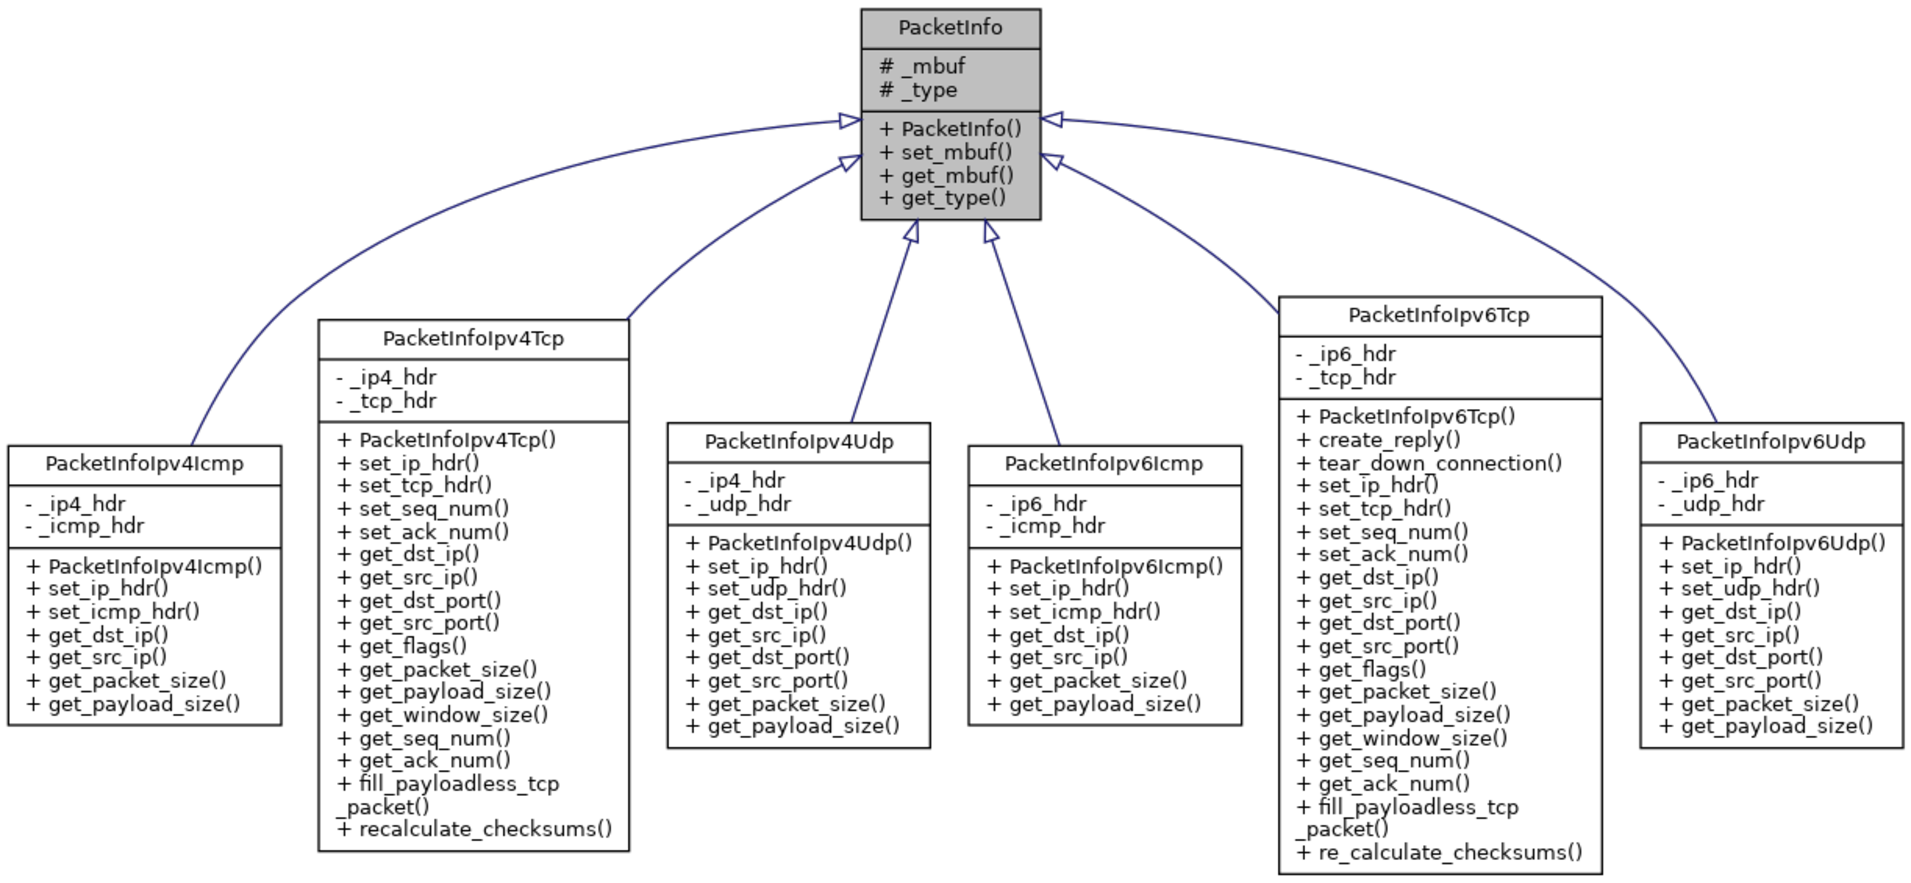
\includegraphics[width=\linewidth]{img/PacketInfoInheritance.pdf}
	\caption{Klassendiagramm aller PacketInfo Varianten}
	\label{Klassendiagramm_PacketInfo}
\end{figure}

\subsection{HeaderExtractor}
Wie bereits erwähnt, wurde die Extraktion der Header Informationen dezentralisiert und wird nur bei Abruf entsprechender Informationen durchgeführt. Dies führte zu einer Verringerung von Code für den HeaderExtractor im Laufe der Entwicklung, weshalb er in den PacketContainer integriert wurde. In obigen Sequenzdiagramm stellt er die Funktionen \textit{extract\_header\_info()} und \textit{fill\_info(rte\_mbuf* mbuf, PacketInfo* pkt\_inf)}.

Dabei wird in \textit{extract\_header\_info()} über die einzelnen Elemente des PacketContainers iteriert und für jeden \texttt{mbuf} die Funktion \textit{fill\_info(rte\_mbuf* mbuf, PacketInfo* pkt\_inf)} aufgerufen. Welche wiederum den PacketInfoCreator ausführt und den \texttt{mbuf} mit der zugehörigen PacketInfo verknüpft.

\subsection{PacketInfoCreator}
Diese Klasse ist ein Hilfsmittel, um Vererbungsketten zu vermeiden. Ihre Aufgabe ist es die zum Paket passende PacketInfo Version zu erzeugen. Dabei ließt der PacketInfoCreator die Layer 3 und Layer 4 Protokoll IDs aus, legt die entsprechenden structs auf den Speicher und speichert sie in der frisch erzeugten PacketInfo.

\section{Inspection}
Die Inspection ist für die Erkennung böswilliger IP Pakete zuständig und untersucht diese daher auf verdächtige Strukturen und Muster. Dazu wird auch eine eigene lokale Statistik erstellt, zur Auswertung genutzt und zur Informationsweitergabe mit einer globalen Statistik geteilt.

Der Initializer erstellt für jeden genutzten Thread eine eigene Inspektion welche alle Pakete dieses Threads analysiert und DDoS Attacken erkennt. Dazu wird der Inspection jeweils ein PacketContainer übergeben, der eine Menge von Paketen enthält, die über das NIC Management eingegangen sind.

Die Erkennung basiert auf einer Mustererkennung von zeitlich aufeinanderfolgenden Paketen nach einer Auftrennung in die Protokolle UDP, TCP und ICMP. UDP und ICMP Pakete werden rein mit einem vorher festgelegten Threshold geprüft, der sich an eine selbst berechnete Angriffsrate anpasst. TCP Pakete werden zusätzlich auf Zero und Small Window sowie auf SYN-FIN und SYN-FIN-ACK Muster überprüft.

Der Ablauf und Reihenfolge der Prüfungen der Inspection ist aus einer Versuchdurchführung mit einem DecisionTree für DDoS-Abwehr enstanden um einen möglichst schnellen und effizienten Ablauf zu finden. Implementiert wurde eine statische, nicht veränderliche Pipeline, die nach größten auzuschließenden Faktoren jedes Pakets vorgeht.

Der Ablauf kann grob in drei Filterstufen, auch Security Layers genannt, unterteilt werden.
\begin{enumerate}
    \item RFC Compliance
    \item Static Rules
    \item Dynamic Rules
\end{enumerate}
Ob ein Paket dem RFC Standard entspricht wird bereits bei der PacketInfo klar. Die Inspection bietet die Möglichkeit, bestimmte Fehler zuzulassen oder Pakete mit bestimmten Fehlern zu blockieren und zu löschen.

Die zweite Stufe der Filter setzt sich aus fest definierten Angriffen und Angriffsmustern zusammen. So sind zum Beispiel bei SYN-FIN und SYN-FIN-ACK Angriffen immer die Flags SYN und FIN oder SYN, FIN und ACK gesetzt, können sofort erkannt und das Paket verworfen werden. Weitere Angriffe die in der statischen Abwehr erkannt werden sind Zero- und Small-Window Angriffe.

In der dynamischen Filterstufe werden die Filterregeln entsprechend dem aktuellen Netzwerkverkehr und vorher eingegangenen Paketen angepasst. So dient ein Limit der Paketrate (engl. Threshold) dazu, UDP und TCP Floods abzuwehren. Eigene Verbindungstabellen der ausgehenden Netzwerkverbindungen lassen jedoch legitime Pakete die als Antwort auf eine bestehende Verbindung dienen weiterhin zu, um den legitimen Netzwerkverkehr nicht einzuschränken.

Die Verknüpfung und Ablauf der Filterung wird in dem folgenden Diagramm vereinfacht dargestellt.
\begin{figure}[h]
    \centering
    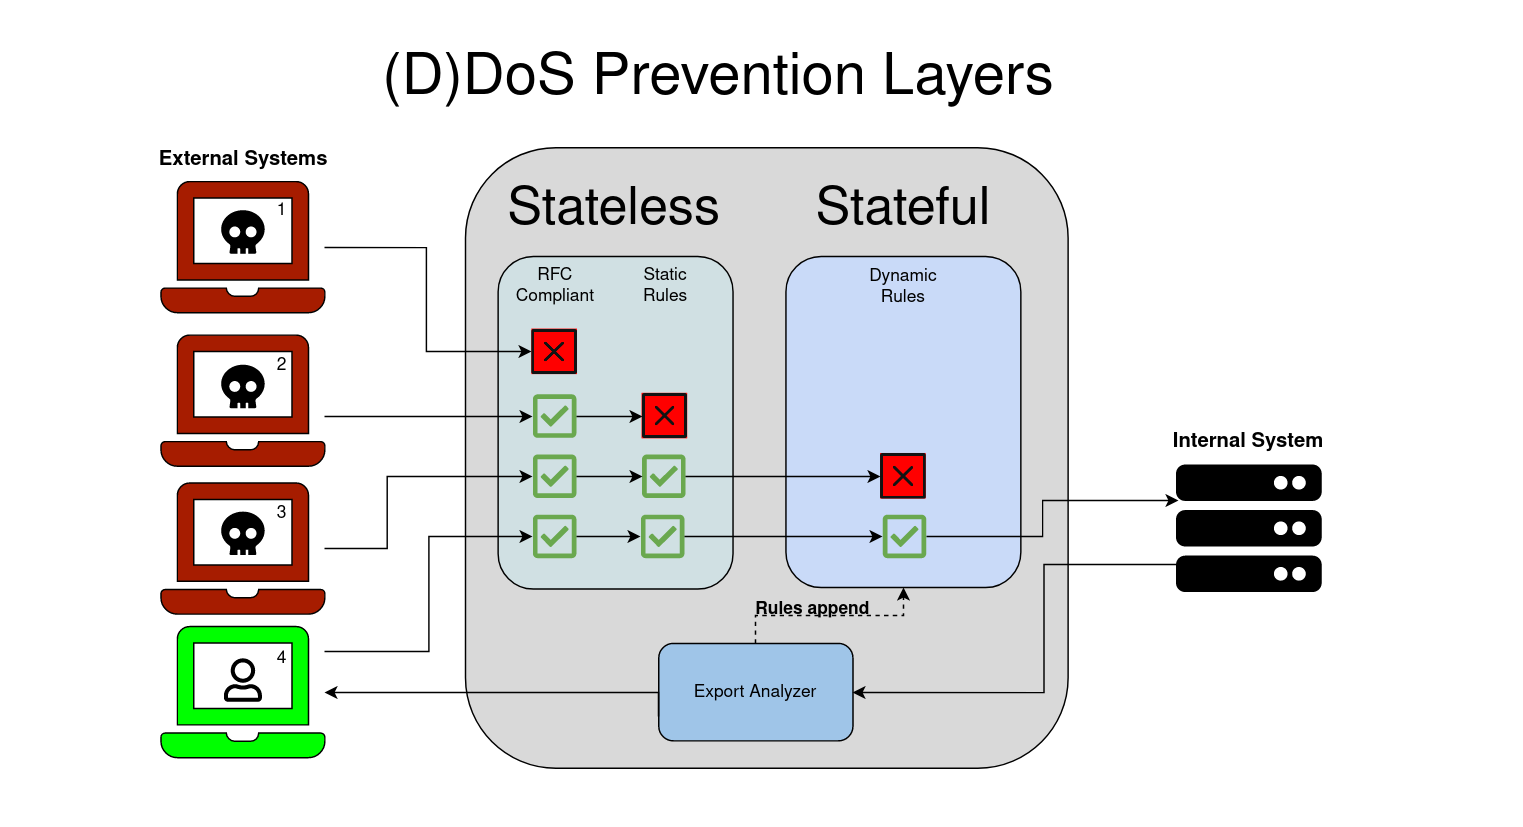
\includegraphics[width=\linewidth]{img/Security_Layers.png}
    \caption{Stufen der Sicherheit}
    \label{security_layers}
\end{figure}

Im Diagramm zu Unterscheiden gilt: die Computer 1 bis 3 sind Angreifer mit unterschiedlichen Angriffen, die ebenso in unterschiedlichen Filterstufen als Angriff erkannt werden und Computer 4 als Nutzer mit legitimen Anfragen an den Server, die den Filterregeln entsprechen.
Ausgehender Verkehr aus dem internen System wird grundsätzlich vertraut und nicht zusätzlich gefiltert. Jedoch wird ausgehender Verkehr analysiert um die dynamischen Regeln anzupassen.

Nach jedem Durchlauf eines PacketContainer werden die lokalen und globalen Statistiken aktualisiert. Die Weitergabe der Informationen an die Statistik erfolgt über einen eigenen interthread Kommunikationskanal zum globalen Statistik-Thread. Die globale Statistik führt alle einzelnen Informationen zusammen und macht sie dem Nutzer in einfacher weise abrufbar.

\begin{figure}[h]
    \centering
    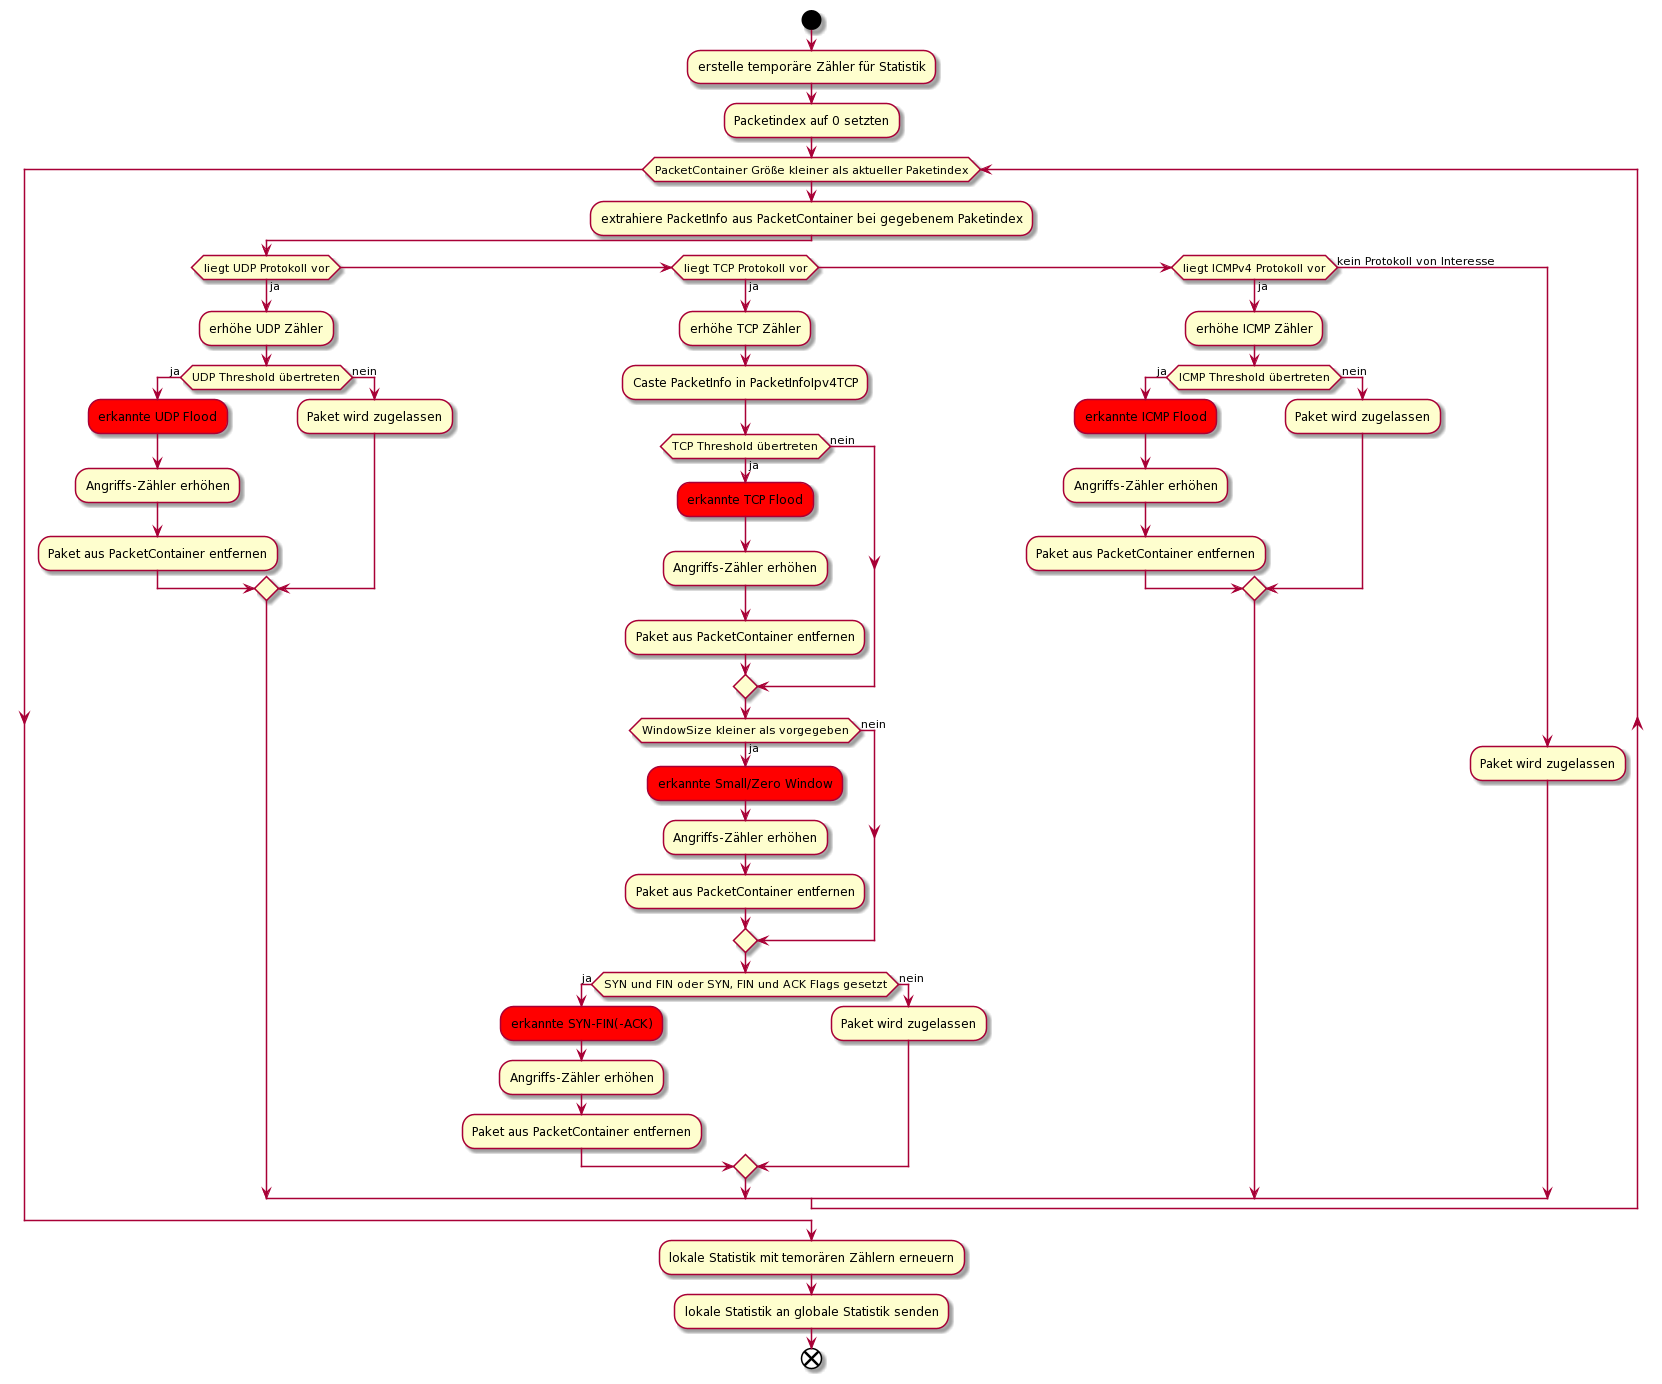
\includegraphics[width=\linewidth]{img/inspection_ablauf.png}
    \caption{Aktivitätsdiagramm der Methode \texttt{analyzePacket()} der Inspection}
    \label{inspection_activity}
\end{figure}


\section{Treatment}

Das \texttt{Treatment}, welches für die Behandlung der SYN-Flut zuständig ist, erhält vom \texttt{Thread} zwei Pointer auf \texttt{PacketContainer}. Für jede Senderichtung, sowohl von Intern nach Extern als auch umgekehrt, existiert einer dieser Container. Der Ablauf in der Behandlung von Paketen unterscheidet sich basierend auf deren Senderichtung. Jedes Paket wird im \texttt{Treatment} zwar einzeln, allerdings im Kontext der gesamten Verbindung betrachtet. Die Behandlung im \texttt{Treatment} beginnt mit dem Iterieren über die Einträge im jeweiligen \texttt{PacketContainer}. Hierbei wird zugleich geprüft, ob das gerade betrachtete Paket bereits gelöscht wurde, oder von einem Typ ist, welcher nicht im \texttt{Treatment} behandelt wird. Dies ist auch im globalen Ablauf der Funktion \texttt{treat\_packets()} in Abbildung \ref{Aktivität_treat_packet_0} sowie \ref{Aktivität_treat_packet_1} zu erkennen. Sollte dies der Fall sein, wird ebendieser Eintrag übersprungen. Sollte es sich bei dem gerade betrachteten Paket beispielsweise um ein UDP Paket handeln, so wird dieses im Treatment nicht weiter betrachtet, da dies bereits im \texttt{Analyzer} geschah. 

Nach diesen ersten Tests findet jeweils eine Fallunterscheidung statt. Für Pakete, welche von extern nach intern geschickt werden sollen, gilt: 

Falls es sich bei dem Paket um ein TCP-SYN-Paket handelt, so wird als Antwort hierauf ein SYN-ACK generiert, dessen Sequenznummer durch einen, vom Programm berechneten, SYN-Cookie ersetzt wird. Hierzu existiert die Methode \texttt{calc\_cookie\_hash()}, welche 24 der 32 Bit langen Sequenznummer generiert, welche später mit 8 Bit Timestamp in der Methode \texttt{treat\_packets()} aufgefüllt werden. Dieser SYN-Cookie enthält Informationen über die Verbindungsentitäten, sowie zur Verbesserung der Effektivität einen Zeitstempel und ein Secret. Dieser SYN-Cookie ermöglicht es, im Verlauf des Verbindungsaufbaus auf das Speichern von Informationen über die Verbindung zu verzichten. Somit wird die Angriffsfläche von SYN-Floods effektiv minimiert. 

Sollte ein ACK als Reaktion auf dieses SYN-ACK erhalten werden, so ist durch die Funktion \texttt{check\_syn\_cookie()} zu überprüfen, ob der empfangene Cookie in Form der Sequenznummer plausibel ist (Siehe Abb. \ref{check_syn_cookie}). Das bedeutet, dass der Zeitstempel maximal eine Zeiteinheit alt ist, welche in diesem Programm 64 Sekunden dauert, und der restliche Cookie mit dem erwarteten Cookie übereinstimmt. Der Cookie setzt sich insgesamt zusammen aus 8 Bit Timestamp, sowie 24 Bit Hashwert über externe und interne IP-Adresse, externe und interne Portnummer sowie dem Timestamp und dem Cookie\_Secret. 
Desweiteren ist eine Verbindung mit dem internen Server, spezifiziert in der DestIP des ACK-Paketes, aufzubauen. Zudem muss die dem ACK hinzugefügten Payload gespeichert werden, auch dies geschieht in einer separaten Map, der ACKmap. Dieses ACK-Paket muss nach erfolgreichem Verbindungsaufbau mit dem internen Server an ebendiesen verschickt werden. 

Wird ein SYN-ACK von extern empfangen, so ist dies ohne Veränderung an das interne Netz zuzustellen. Allerdings muss hier ein Eintrag in der Offsetmap erzeugt werden, wobei der Offset realisierungsbedingt null ist. 

Werden Pakete ohne gesetzte Flags, beziehungsweise nur mit gesetztem ACK-Flag verschickt, so findet eine Sequenznummernzuordnung und eine Anpassung von Sequenznummern statt. Hierzu wird eine Densemap mit individueller Hashfunktion, in diesem Fall XXH3, verwendet. Bei der Densemap handelt es sich um eine besonders effiziente Hashmap, welche ein Einfügen, Suchen und Löschen in bis zu vier mal weniger Zeit als eine unordered\_map ermöglicht. Die Auswahl der Hashfunktion XXH3 ist  dadurch motiviert, dass sie extrem schnell ist und dennoch kaum Kollisionen erzeugt. Insbesondere werden durch sie bereits auf handelsüblichen Computersystemen Hashraten von bis zu 31.5 Gbit/s erzielt.
 
Der Ablauf bei Empfang eines solchen Paketes ist wie folgt: Bei eingehenden Paketen wird ein zuvor berechneter Offset, welcher in der Offsetmap für jede Verbindung gespeichert ist, von der ACK-Nummer subtrahiert.

Wird ein ACK empfangen, welches zu einer Verbindung gehört, in deren Info finseen auf true gesetzt ist, so muss die ACK-Nummer angepasst, das Paket an den internen Server geschickt und der Eintrag in der Densemap verworfen werden.  
  
Falls ein Paket mit gesetzem RST-Flag von extern empfangen wird, wird der Eintrag in der Densemap gelöscht und das empfangene Paket an den internen Server weitergeleitet. Hierbei muss keine Anpassung der ACK-Nummer vorgenommen werden.
 
Sollte ein FIN empfangen werden, so muss im Info-Struct, welches Teil der Offsetmap ist, der Wert finseen auf true gesetzt werden. In diesem Fall ist das Paket nach Anpassung der ACK-Nummer weiterzuleiten.



Im zweiten Fall der übergeordneten Fallunterscheidung erhält das Programm den \texttt{PacketContainer} der Pakete, welche das Netz von intern nach extern verlassen wollen. Auch hier wird, bevor ein Paket der Behandlung unterzogen wird, geprüft, ob das Paket nicht bereits gelöscht wurde, oder es sich um ein Paket falschen Typs handelt. 

Falls ein Paket mit gesetzem RST-Flag von extern empfangen wird, wird der Eintrag in der Densemap gelöscht und das empfangene Paket an den internen Server weitergeleitet. Hierbei muss keine Anpassung der ACK-Nummer vorgenommen werden.

Sollte ein FIN empfangen werden, so muss im Info-Struct, welches Teil der Offsetmap ist, der Wert finseen auf true gesetzt werden. In diesem Fall ist das Paket nach Anpassung der ACK-Nummer weiterzuleiten.



Im zweiten Fall der übergeordneten Fallunterscheidung erhält das Programm den \texttt{PacketContainer} der Pakete, welche das Netz von intern nach extern verlassen wollen. Auch hier wird, bevor ein Paket der Behandlung unterzogen wird, geprüft, ob das Paket nicht bereits gelöscht wurde, oder es sich um ein Paket falschen Typs handelt.

Erhält das System ein SYN-Paket von einem internen Server, so wird dieses an das im Paket spezifizierte Ziel weitergeleitet. Eine Anpassung der Sequenznummer findet in diesem Fall nicht statt.

Erhält das System ein SYN-ACK aus dem internen Netz, so muss das System die Differenz aus der ACK-Nummer dieses Pakets, und der des in der ACKmap gespeicherten Paketes berechnen, und den Wert als Offset in der Offsetmap eintragen. Das von intern empfangene SYN-ACK Paket muss verworfen werden.
Das zuvor in der ACKmap zwischengespeicherte Paket muss nun mit angepasster ACK-Nummer intACK = extACK-offset an den internen Host geschickt werden.

Wird ein Paket ohne gesetzte Flags oder mit gesetztem ACK-Flag von Intern nach Extern verschickt, so findet eine weitere Fallunterscheidung statt.
Im Fall, dass finseen bereits auf true gesetzt ist, muss der Offset in der Offsetmap nachgeschlagen werden, der Eintrag daraufhin gelöscht werden und das empfangene Paket mit extSeq = intSeq + offset verschickt werden.
Gesetzt den Fall, dass noch kein Eintrag in der Offsetmap existiert, muss ein neuer Eintrag in dieser erstellt werden. Der Offsetwert muss auf null, und finseen auf false gesetzt werden. Das empfangene Paket muss hiernach nach Intern weitergeleitet werden.
Trifft keiner der beiden obigen Fälle ein, so muss der Offset in der Offsetmap nachgeschlagen werden und das empfangene Paket nach Intern weitergeschickt werden. Vor dem Versenden muss hierbei die Sequenznummer wie folgt angepasst werden: extSeq = intSeq + offset.

Sollte ein Paket mit gesetzem FIN-Flag erkannt werden, so ist diese Information in der Info an Stelle Key = Hash(extip, intip, extport, intport) mit dem Vermerk finseen = true, zu speichern. Das empfangene Paket ist durch das System nach extern mit extSeq = intSeq + offset weiterzuschicken.

Wird ein RST erhalten, so ist eine Anpassung der Sequenznummer vorzunehmen, das Paket entsprechend weiterzuleiten und der Eintrag in der Offsetmap an entsprechender Stelle zu entfernen.

Desweiteren könnte es unter Umständen erforderlich werden, die Einträge mit einem Timestamp zu versehen, welcher speichert, wann dieser Eintrag zuletzt verwendet wurde, sollte es zu Situationen kommen, in denen sowohl Sender als auch Empfänger die Verbindung nicht korrekt terminieren können. Dies ist bisweilen allerdings nicht implementiert, die Idee wird allerdings basierend auf den Ausgängen der Tests auf dem Testbed weiter verfolgt oder verworfen.

\begin{figure}[h]
    \centering
    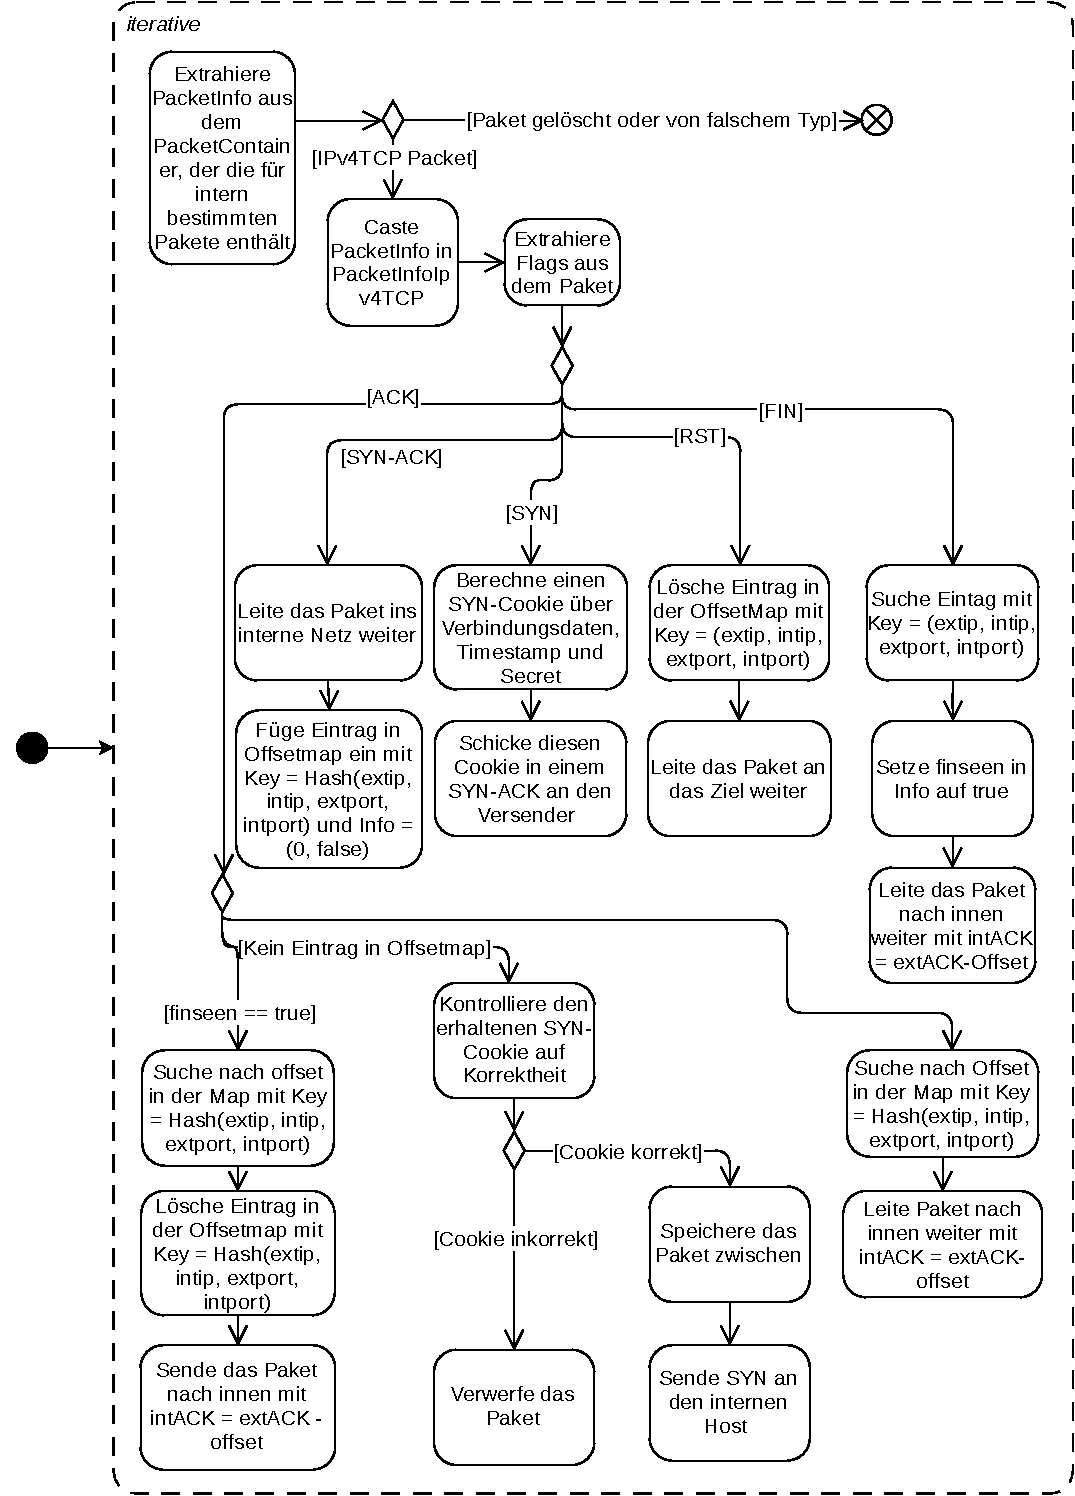
\includegraphics[width=0.98\linewidth]{img/treat_packets_0.pdf}
    \caption{Aktivitätsdiagramm der Methode \texttt{treat\_packets()}, Teil: Pakete nach Intern}
    \label{Aktivität_treat_packet_0}
\end{figure}
\begin{figure}[h]
	\centering
	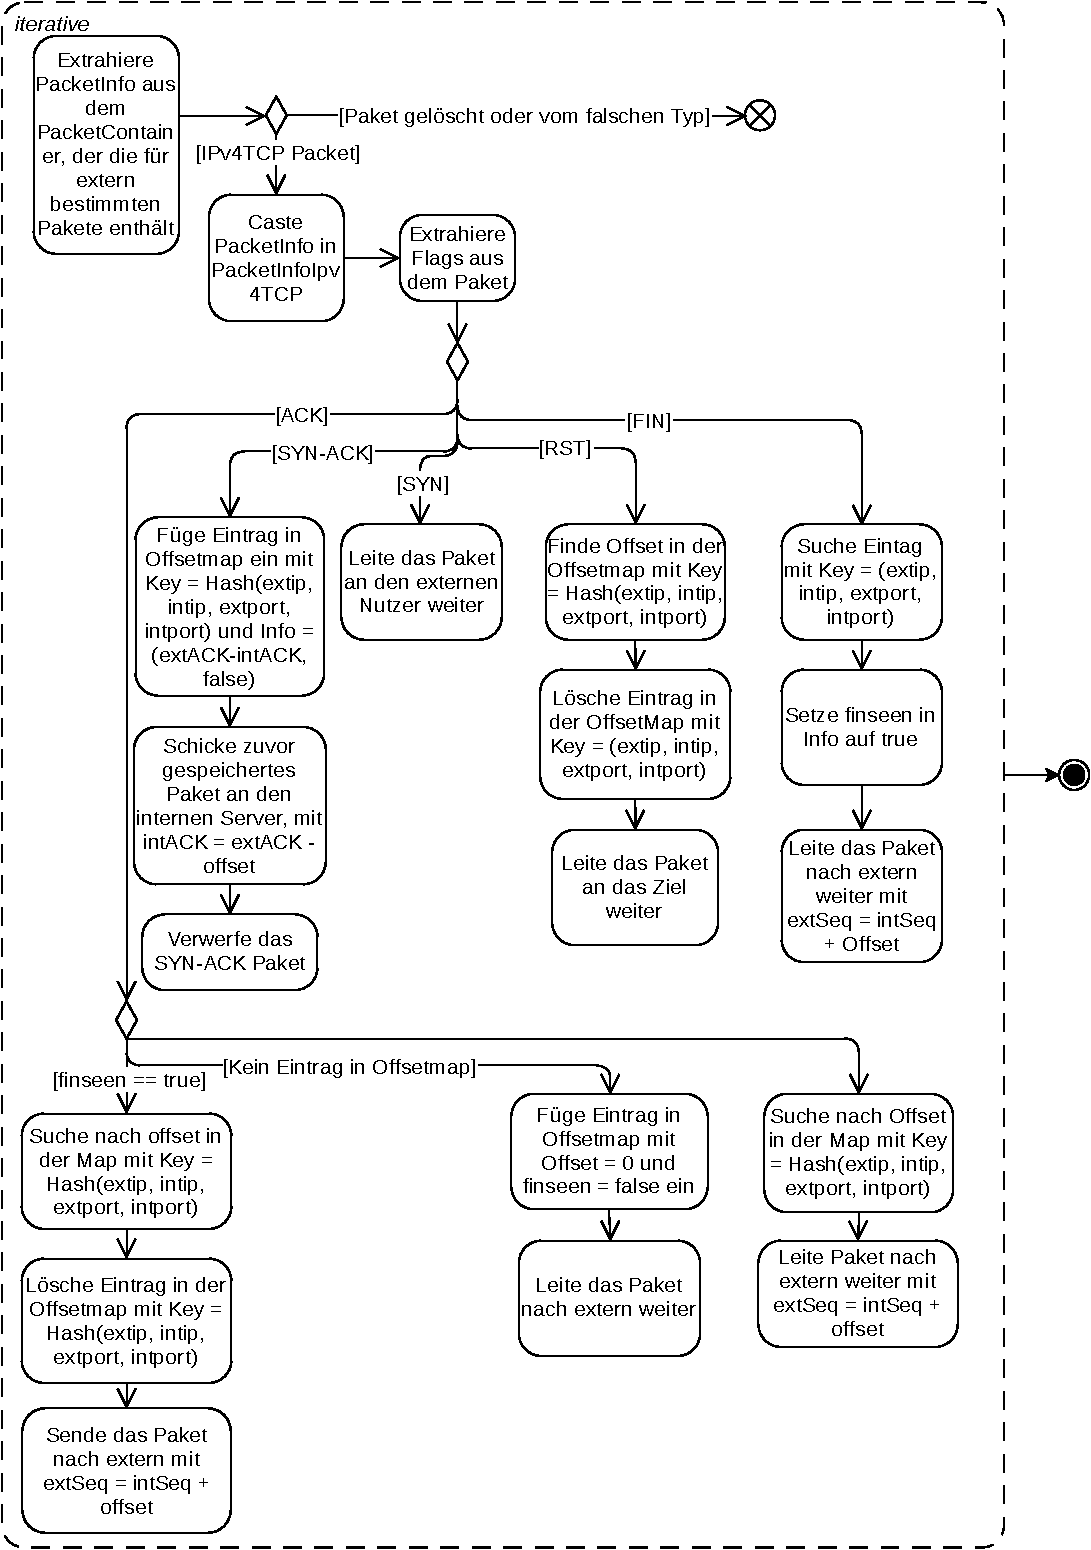
\includegraphics[width=0.96\linewidth]{img/treat_packets_1.pdf}
	\caption{Aktivitätsdiagramm der Methode treat\_packets(), Teil: Pakete nach Extern}
	\label{Aktivität_treat_packet_1}
\end{figure}

\begin{figure}[t]
    \centering
    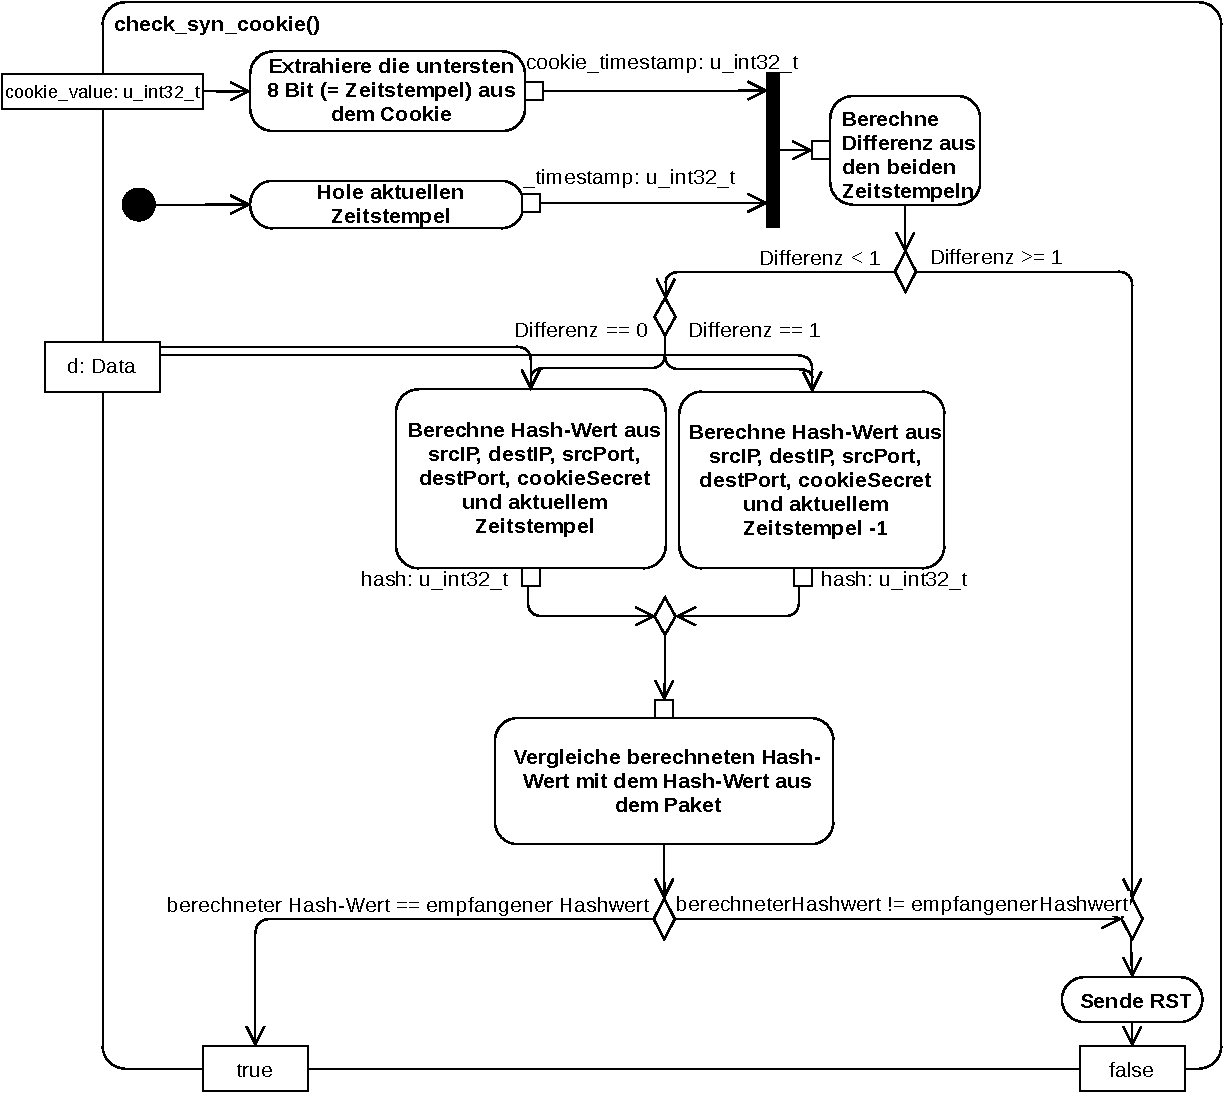
\includegraphics[width=\linewidth]{img/check_typ_syn_cookie_neu.pdf}
    \caption{Aktivitätsdiagramm der Methode check\_syn\_cookie()}
    \label{check_syn_cookie}
\end{figure}
    Nachdem ein ACK als Reaktion auf ein SYN-ACK bei dem zu entwerfenden System angekommen ist, wird die Methode \texttt{check\_typ\_syn\_cookie()} aufgerufen.
    Grundsätzlich wird hier überprüft, ob der Hash-Wert aus dem empfangenen Paket mit dem eigens berechneten Hash-Wert übereinstimmt. Falls dies nicht der Fall ist oder die Differenz der Zeitstempel zu groß ist, wird ein Paket mit gesetzten Reset-Flag (RST) an den Sender geschickt. Dieses Flag zeigt an, dass die Verbindung beendet werden soll. Andernfalls wird die Verbindung als legitim erkannt und das Paket in der ACKmap zwischengespeichert, bis die Verbindung mit dem internen System erfolgreich war. 
    

\begin{figure}[t]
    \centering
    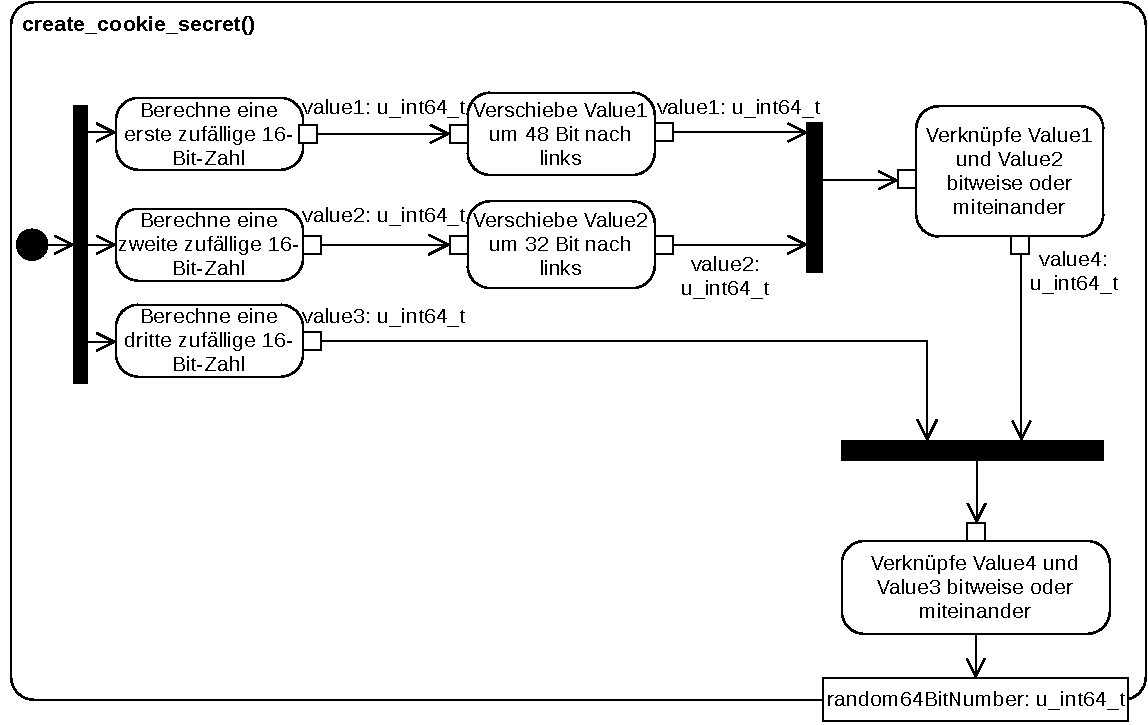
\includegraphics[width=\linewidth]{img/create_cookie_secret_neu.pdf}
    \caption{Aktivitätsdiagramm der Methode \textit{create\_cookie\_secret()}}
    \label{createcookiesecret}
\end{figure}
Abbildung \ref{createcookiesecret} zeigt die parameterlose Methode \texttt{create\_cookie\_secret()}. Zu Beginn werden drei 16-Bit lange Zufallszahlen generiert, wobei auf cie Funktion \textit{rand()} aus der C Standardbibliothek zugegriffen wird. Der erste mit \texttt{rand()} generierte Wert wird um 48 Bit nach links verschoben, der zweite um 32 Bit. Diese beiden Werte werden danach bitweise ODER miteinander verknüpft. Dieser verknüpfte Wert wird dann wiederum mit der dritten zufälligen 16-Bit Zahl bitweise ODER verknüpft. Das Ergebnis dieser Verknüpfung ist eine 64-Bit lange Zufallszahl, die von der Methode zurückgegeben wird.

\end{document}
